\documentclass[10pt,journal,compsoc]{IEEEtran}

\usepackage[utf8]{inputenc}
\usepackage{amsmath,amssymb,amsfonts}
\usepackage{algorithmic}
\usepackage{graphicx}
\usepackage{textcomp}
\usepackage{xcolor}
\usepackage{booktabs}
\usepackage{multirow}
\usepackage{microtype}
\usepackage{hyperref}
\usepackage{url}
\usepackage{cite}

\hypersetup{
    colorlinks=true,
    linkcolor=blue!70!black,
    citecolor=green!50!black,
    urlcolor=blue!80!black
}

\begin{document}

\title{Card Fraud Triage via Gaussian Mixture Density Scoring and Unsupervised Anomaly Detection}

\author{Ritik~Ranjan,
        Archit~Mamodiya,
        Shagun~Vishnoi,
        Aditya~Raj,
        and~Naveen~Kumar%
\IEEEcompsocitemizethanks{
\IEEEcompsocthanksitem Team ID: T047, Section A, Project 26.\protect\\
Applied Machine Learning (Phase 1 Baseline Technical Report).
}}

\markboth{AML Project 26: Card Fraud Triage via Density Scoring, October~2026}%
{Team T047: Card Fraud Triage via Gaussian Mixture Density Scoring}

\IEEEtitleabstractindextext{%
\begin{abstract}
Financial card fraud detection in production banking environments faces severe class imbalance ($\sim 0.17\%$), delayed ground-truth verification labels (often 30--90 days), and strict limits on human investigation capacity. While supervised classifiers degrade when fraud topologies evolve, unsupervised density estimation provides an operational triage filter by modelling purely legitimate consumer behavior. In this Phase~1 study, we investigate whether a Gaussian Mixture Model (GMM) trained exclusively on normal transactions can effectively rank fraudulent swipes for manual triage under realistic operational constraints. Using the benchmark ULB European cardholder dataset (283,726 deduplicated transactions across 48 hours), we enforce strict temporal integrity via a 60/20/20 chronological split. Feature distributions reject univariate normality ($p < 10^{-100}$), confirming multimodality. Training exclusively on 169,893 normal transactions from the first 60\% of time, we execute an extensive grid search across component counts ($K=1$ to $8$) and random initialisations. The champion configuration ($K=3$, Full Covariance, 29 features) achieves an Average Precision (AP) of 0.612 (95\% bootstrap CI [0.485, 0.743]) on the completely unseen test period, outperforming the random-guess baseline (0.0013) by 470$\times$. At an operational false-positive rate budget fixed at $\le 0.5\%$ on validation ($\tau = 94.68$), the model intercepts 56 of 74 test frauds (75.7\% Recall) with only 158 false alarms (0.28\% FPR). In human review triage scenarios, the top 50 flagged transactions achieve an alert precision of 84.0\% (42 confirmed frauds). Our empirical findings demonstrate that full-covariance mixture models capture subtle multivariate cross-correlations that univariate feature selection discards, establishing an unsupervised baseline for ongoing Phase~2 autoencoder research.
\end{abstract}

\begin{IEEEkeywords}
Fraud detection, unsupervised anomaly detection, Gaussian mixture models, expectation-maximization, class imbalance, precision-recall curve, operational triage.
\end{IEEEkeywords}}

\maketitle
\IEEEdisplaynontitleabstractindextext
\IEEEpeerreviewmaketitle

\section{Introduction}
\IEEEPARstart{C}{redit} card fraud accounts for tens of billions of dollars in annual global losses, posing an existential challenge to financial payment processors and consumer banking infrastructure~\cite{dalpozzolo2018credit}. The technical challenge of building effective automated fraud defense mechanisms stems from three fundamental characteristics of transactional data:
\begin{enumerate}
    \item \textbf{Extreme Class Imbalance:} Fraudulent activities constitute a minuscule fraction of daily volume (typically under $0.2\%$). Standard accuracy metrics are trivialized, as a static null classifier predicting all transactions as legitimate achieves $>99.8\%$ accuracy while failing completely.
    \item \textbf{Delayed Verification Ground Truth:} In production environments, fraud labels are not immediately available. Fraud is typically reported weeks later via chargebacks, merchant reconciliations, or customer disputes~\cite{carcillo2018scarff}. Supervised classifiers that require contemporaneous labels suffer severe degradation under operational delay.
    \item \textbf{Analyst Capacity Constraints:} Security operations centers (SOCs) have finite human review bandwidth. An algorithm generating thousands of low-confidence alerts overwhelms fraud investigation personnel, leading to alert fatigue and high operational costs.
\end{enumerate}

To circumvent the latency of supervised label acquisition, unsupervised anomaly detection provides a compelling alternative~\cite{chandola2009anomaly}. By training a density model strictly on abundant, verified historical legitimate purchases, the system establishes a probabilistic boundary of normal cardholder behavior. When incoming transactions exhibit low likelihood under the learned distribution, they receive high anomaly scores and are triaged into an analyst priority queue.

In this work (Phase~1 of Project~26), we develop and empirically validate an unsupervised fraud triage system utilizing Gaussian Mixture Models (GMM). We formulate anomaly detection through negative log-likelihood (NLL) density scoring. We evaluate our pipeline on the ULB credit card benchmark under a time-ordered chronological split, comparing full feature representations against dimensionality-reduced candidate sets.

\section{Related Work}
Machine learning in credit card fraud detection has evolved across multiple paradigms. Dal Pozzolo et al.~\cite{dalpozzolo2015calibrating, dalpozzolo2018credit} formalized the benchmark evaluation framework for card fraud, proving that random $k$-fold cross-validation introduces severe temporal lookahead leakage and inflates performance metrics. They established that chronological partitioning and human verification capacity metrics ($P@k$) are mandatory for realistic assessment.

Unsupervised anomaly detection has been surveyed comprehensively by Chandola et al.~\cite{chandola2009anomaly}. Classical methods include distance-based algorithms ($k$-NN, Local Outlier Factor), linear projections (PCA reconstruction), and parametric density models. Gaussian Mixture Models, optimized via Expectation-Maximization (EM)~\cite{bishop2006pattern}, offer analytical density evaluations and capture multimodal consumer spending habits through heterogeneous component centers and full covariance matrices.

Davis and Goadrich~\cite{davis2006relationship} established that under massive class skew, the Receiver Operating Characteristic (ROC) curve is structurally flattered by the overwhelming volume of True Negatives. They demonstrated that Precision-Recall (PR) curves and Average Precision (AP) provide an uncompromised assessment of minority-class retrieval.

Recent advancements explore deep autoencoding architectures~\cite{sakurada2014anomaly} and deep autoencoding Gaussian mixture models (DAGMM)~\cite{zong2018deep}, which unify dimensionality reduction and density estimation. Our Phase~1 GMM baseline establishes the mathematical benchmark against which Phase~2 autoencoders will be contrasted.

\section{Dataset and Chronological Partitioning}
\subsection{Dataset Properties}
We utilize the public European cardholder benchmark dataset collected by the Machine Learning Group at Universit{\'e} Libre de Bruxelles (ULB)~\cite{dalpozzolo2015calibrating}. The dataset contains 284,807 transactions recorded over a continuous 48-hour period in September 2013, with 492 confirmed fraudulent events ($0.173\%$ prevalence).

The dataset consists of 30 numerical input features:
\begin{itemize}
    \item \texttt{Time}: Elapsed time in seconds from the first recorded transaction.
    \item \texttt{Amount}: Transaction value denominated in Euros.
    \item \texttt{V1}--\texttt{V28}: Anonymized continuous numerical attributes derived from a proprietary Principal Component Analysis (PCA) performed by the banking institution for data privacy.
    \item \texttt{Class}: Binary ground truth ($0 = \text{Legitimate}, 1 = \text{Fraud}$).
\end{itemize}

\subsection{Deduplication and Leakage-Safe Time Split}
Data auditing identified 1,081 exact duplicate rows (including 19 fraudulent records), which were purged to prevent artificial density inflation, leaving 283,726 clean rows.

\begin{table}[t]
\centering
\caption{Chronological Data Partitioning (60 / 20 / 20 Split)}
\label{tab:datasplit}
\begin{tabular}{lcccc}
\toprule
\textbf{Split} & \textbf{Time Window} & \textbf{Total Rows} & \textbf{Frauds} & \textbf{Prevalence} \\
\midrule
Train & First 60\% ($0 - 28.8\text{ h}$) & 169,893 & 0 (342 rem.) & 0.000\% \\
Validation & Next 20\% ($28.8 - 38.4\text{ h}$) & 56,745 & 57 & 0.100\% \\
Test & Last 20\% ($38.4 - 48.0\text{ h}$) & 56,746 & 74 & 0.130\% \\
\bottomrule
\end{tabular}
\end{table}

To prevent temporal data leakage, we enforce a strict 60/20/20 chronological partition based on \texttt{Time} (Table~\ref{tab:datasplit}):
\begin{enumerate}
    \item \textbf{Training Period (First 60\%):} 170,235 transactions. All 342 fraud records occurring in this window are removed. The remaining 169,893 purely legitimate transactions are used to fit the standard scaler and the unsupervised GMM.
    \item \textbf{Validation Period (Next 20\%):} 56,745 transactions (57 frauds, $0.100\%$ rate). Used to optimize hyperparameters ($K$, covariance constraints, random seeds) and tune the operational decision threshold.
    \item \textbf{Test Period (Final 20\%):} 56,746 transactions (74 frauds, $0.130\%$ rate). Kept strictly sealed until model finalization for unbiased out-of-time evaluation.
\end{enumerate}

\section{Exploratory Data Analysis and Feature Engineering}
To ensure methodological hygiene, all exploratory analysis and feature ranking are conducted exclusively on the training period without peeking at validation or test labels.

\subsection{Diurnal Transaction Distributions}
We derive transaction hour as:
\begin{equation}
\text{Hour} = \left\lfloor \frac{\text{Time}}{3600} \right\rfloor \pmod{24}
\end{equation}
As illustrated in Fig.~\ref{fig:diurnal}, normal transaction volume exhibits strong diurnal rhythm, dropping significantly between 01:00 and 06:00. Conversely, fraudulent swipes remain active during nocturnal hours, spiking between 02:00 and 04:00 where detection friction is minimal.

\begin{figure}[t]
\centering
\includegraphics[width=0.95\linewidth]{../results/figures/fig1_time_diurnal_distribution.png}
\caption{Diurnal transaction volume distribution (Normal vs. Fraud) during the training period, demonstrating nocturnal fraud concentration.}
\label{fig:diurnal}
\end{figure}

\begin{figure}[t]
\centering
\includegraphics[width=0.95\linewidth]{../results/figures/fig2_amount_distribution_log.png}
\caption{Distribution of transaction \texttt{Amount}: Raw distribution exhibits extreme right-skew ($\gamma_1 = 15.77$), while $\log(1 + \text{Amount})$ normalizes the profile ($\gamma_1 = 0.16$).}
\label{fig:amount_log}
\end{figure}

\subsection{Amount Log-Transformation}
Raw purchase amounts span from \texteuro0.00 to \texteuro25,691.16 with a median of \texteuro22.00, yielding extreme positive skewness ($\gamma_1 = 15.77$). To accommodate the Gaussian structural assumptions of our mixture components, we apply a natural logarithmic transformation:
\begin{equation}
\widetilde{\text{Amount}} = \ln(1 + \text{Amount})
\end{equation}
Fig.~\ref{fig:amount_log} verifies that the transformation reduces skewness to $\gamma_1 = 0.16$, yielding an approximately bell-shaped distribution suitable for GMM covariance estimation.

\subsection{Feature Divergence Analysis (KS Test)}
To identify the most discriminative features, we compute the two-sample Kolmogorov-Smirnov (KS) statistic~\cite{massey1951kolmogorov} between normal and fraudulent training distributions:
\begin{equation}
D_{KS} = \sup_x |F_{\text{normal}}(x) - F_{\text{fraud}}(x)|
\end{equation}
The top 11 divergent features ($V14, V10, V12, V11, V17, V4, V3, V16, V7, V2, V9$) all exhibit $D_{KS} > 0.32$ (Fig.~\ref{fig:kde}). These 11 features, combined with $\widetilde{\text{Amount}}$, form our candidate 12-feature subset recorded in \texttt{configs/gmm_features.json}.

\begin{figure}[t]
\centering
\includegraphics[width=0.98\linewidth]{../results/figures/fig3_top_divergent_features_kde.png}
\caption{Kernel density estimations for the top six separating features identified by the two-sample Kolmogorov-Smirnov test.}
\label{fig:kde}
\end{figure}

\begin{figure}[t]
\centering
\includegraphics[width=0.88\linewidth]{../results/figures/fig4_feature_correlation_matrix.png}
\caption{Correlation matrix of Hour, Amount, and top separating PCA features.}
\label{fig:correlation}
\end{figure}

\subsection{Multimodality and Normality Rejection}
We applied the D'Agostino-Pearson omnibus test~\cite{dagostino1973tests} on legitimate transactions for \texttt{Amount}, $V1$, $V4$, and $V14$. Every tested feature yielded $p$-values $< 10^{-100}$, rejecting unimodal Gaussian behavior. Legitimate consumer spending consists of distinct behavioral personas (e.g., micro-purchases, recurring utilities, commercial corporate cards), necessitating a multi-component mixture model.

\section{Methodology: Gaussian Mixture Density Scoring}
\subsection{Mathematical Formulation}
A Gaussian Mixture Model models the probability density function of continuous feature vector $x \in \mathbb{R}^D$ as a convex combination of $K$ multivariate Gaussian distributions:
\begin{equation}
p(x \mid \theta) = \sum_{k=1}^{K} \pi_k \mathcal{N}(x \mid \mu_k, \Sigma_k)
\end{equation}
subject to mixing proportions $\sum_{k=1}^K \pi_k = 1$ ($\pi_k \ge 0$), where component density is defined as:
\begin{equation}
\mathcal{N}(x \mid \mu_k, \Sigma_k) = \frac{\exp\left(-\frac{1}{2}(x - \mu_k)^T \Sigma_k^{-1} (x - \mu_k)\right)}{(2\pi)^{D/2} |\Sigma_k|^{1/2}}
\end{equation}

Model parameters $\theta = \{\pi_k, \mu_k, \Sigma_k\}_{k=1}^K$ are estimated on the unlabelled legitimate training set $X_{\text{train}}$ via the Expectation-Maximization (EM) algorithm~\cite{bishop2006pattern}:
\begin{itemize}
    \item \textbf{E-Step:} Compute posterior responsibilities:
    \begin{equation}
    \gamma_{ik} = \frac{\pi_k \mathcal{N}(x_i \mid \mu_k, \Sigma_k)}{\sum_{j=1}^K \pi_j \mathcal{N}(x_i \mid \mu_j, \Sigma_j)}
    \end{equation}
    \item \textbf{M-Step:} Update component weights, centroids, and covariance matrices:
    \begin{align}
    N_k &= \sum_{i=1}^N \gamma_{ik}, \quad \pi_k = \frac{N_k}{N}, \quad \mu_k = \frac{1}{N_k} \sum_{i=1}^N \gamma_{ik} x_i \\
    \Sigma_k &= \frac{1}{N_k} \sum_{i=1}^N \gamma_{ik} (x_i - \mu_k)(x_i - \mu_k)^T + \epsilon I
    \end{align}
    where regularisation covariance $\epsilon = 10^{-5}$ is added to diagonals to prevent numerical singularity.
\end{itemize}

\subsection{Anomaly Scoring Function}
For any incoming transaction $x$, the GMM evaluates the likelihood of legitimate generation. Transactions residing in low-density probability regions reflect anomalous behavioral deviations. We compute the anomaly score $S(x)$ as the Negative Log-Likelihood (NLL):
\begin{equation}
S(x) = -\ln p(x \mid \hat{\theta}) = -\ln \left( \sum_{k=1}^K \hat{\pi}_k \mathcal{N}(x \mid \hat{\mu}_k, \hat{\Sigma}_k) \right)
\end{equation}
High values of $S(x)$ trigger security triage alerts.

\subsection{Hyperparameter Grid and Model Selection Protocol}
The search space evaluated:
\begin{itemize}
    \item Feature Sets: All 29 features ($V1$--$V28$ + $\widetilde{\text{Amount}}$) vs. Selected 12 features.
    \item Mixture Components: $K \in \{1, 2, 3, 4, 5, 6, 7, 8\}$.
    \item EM Restarts and Stability: To overcome local optima in non-convex EM log-likelihood surfaces, each model was fitted with $n\_init = 5$ across 3 distinct random seeds ($\{0, 1, 2\}$), totaling 144 fitted models executed in parallel.
\end{itemize}

Candidate configurations were ranked by mean validation Average Precision (AP). The Bayesian Information Criterion (BIC), defined as:
\begin{equation}
\text{BIC} = p \ln(N) - 2 \ln(\hat{L})
\end{equation}
where $p$ is the number of free parameters and $\hat{L}$ is maximized likelihood, was monitored for complexity penalization.

\begin{figure}[t]
\centering
\includegraphics[width=0.98\linewidth]{../results/figures/fig5_gmm_component_selection.png}
\caption{Hyperparameter search across component count $K$: (Left) BIC trajectories; (Right) Validation Average Precision across random seeds.}
\label{fig:component_selection}
\end{figure}

\begin{table}[t]
\centering
\caption{Validation Performance Across Feature Sets and $K$ Components}
\label{tab:gmm_results}
\begin{tabular}{lccccc}
\toprule
\textbf{Features} & $\mathbf{K}$ & \textbf{AP Mean} & \textbf{AP Min} & \textbf{AP Max} & \textbf{Mean BIC} \\
\midrule
All 29 & 1 & 0.074 & 0.074 & 0.074 & 13,701,380 \\
All 29 & 2 & 0.176 & 0.079 & 0.371 & 6,635,476 \\
\textbf{All 29} & \textbf{3} & \textbf{0.549} & \textbf{0.343} & \textbf{0.666} & \textbf{3,412,903} \\
All 29 & 4 & 0.068 & 0.065 & 0.074 & -1,218,040 \\
All 29 & 5 & 0.300 & 0.058 & 0.647 & -2,666,021 \\
All 29 & 6 & 0.068 & 0.059 & 0.078 & -3,176,066 \\
All 29 & 7 & 0.196 & 0.128 & 0.232 & -3,987,216 \\
All 29 & 8 & 0.323 & 0.246 & 0.419 & -5,122,966 \\
\midrule
Selected 12 & 1 & 0.266 & 0.266 & 0.266 & 5,643,466 \\
Selected 12 & 2 & 0.205 & 0.201 & 0.213 & 4,670,746 \\
Selected 12 & 3 & 0.201 & 0.199 & 0.205 & 4,387,461 \\
Selected 12 & 4 & 0.197 & 0.197 & 0.198 & 4,047,104 \\
Selected 12 & 5 & 0.203 & 0.198 & 0.212 & 3,833,669 \\
Selected 12 & 6 & 0.334 & 0.081 & 0.628 & 3,628,444 \\
Selected 12 & 7 & 0.067 & 0.065 & 0.069 & 3,297,546 \\
Selected 12 & 8 & 0.075 & 0.065 & 0.095 & 3,158,924 \\
\bottomrule
\end{tabular}
\end{table}

\section{Experimental Results and Discussion}
\subsection{Validation Grid Search Findings}
As summarized in Table~\ref{tab:gmm_results} and Fig.~\ref{fig:component_selection}:
\begin{enumerate}
    \item \textbf{Failure of Likelihood-Based Penalization (BIC):} For All 29 features, BIC decreases monotonically and turns negative for $K \ge 4$. This occurs because individual Gaussian components collapse onto localized dense transaction pockets, inflating likelihood without improving generalizable fraud separation. Model selection must rely on task-specific validation AP rather than BIC.
    \item \textbf{Dimensionality vs. Flexibility Trade-off:} At $K=1$, the Selected 12 features outperform All 29 ($\text{AP} = 0.266$ vs. $0.074$), as a single unimodal Gaussian suffers from the curse of dimensionality over 29 features. However, at $K=3$, the All 29 feature set achieves the peak performance of the study ($\text{AP}_{\text{mean}} = 0.549$, peak seed $\text{AP} = 0.6661$). The $29 \times 29$ full covariance matrix captures 406 pairwise joint correlations that univariate feature ranking discarded.
    \item \textbf{EM Solution Variance:} GMM quality varies substantially with initialization seed. For All 29 at $K=3$, AP ranges from 0.343 to 0.666 across seeds, reinforcing the necessity of multi-seed evaluations.
\end{enumerate}

The champion configuration selected for test deployment is: \textbf{All 29 features, $K=3$, Full Covariance, Seed 2} (Validation $\text{AP} = 0.6661$).

\subsection{Operational Decision Thresholding}
To translate continuous anomaly scores into automated binary decisions, the operational threshold $\tau$ was calibrated on the validation set under \textbf{Scenario A: False Alarm Budget}:
\begin{equation}
\tau = \text{Percentile}_{99.5} \left( \{ S(x) \mid x \in X_{\text{val}}, y = 0 \} \right) = 94.68
\end{equation}
This policy guarantees that $\ge 99.5\%$ of legitimate cardholders experience uninterrupted service ($\le 0.5\%$ FPR).

\begin{figure}[t]
\centering
\includegraphics[width=0.98\linewidth]{../results/figures/fig6_gmm_test_pr_curve.png}
\caption{Precision-Recall Curve on the held-out test set ($\text{AP} = 0.6121$), operating at 470$\times$ the random baseline ($0.13\%$).}
\label{fig:pr_curve}
\end{figure}

\begin{figure}[t]
\centering
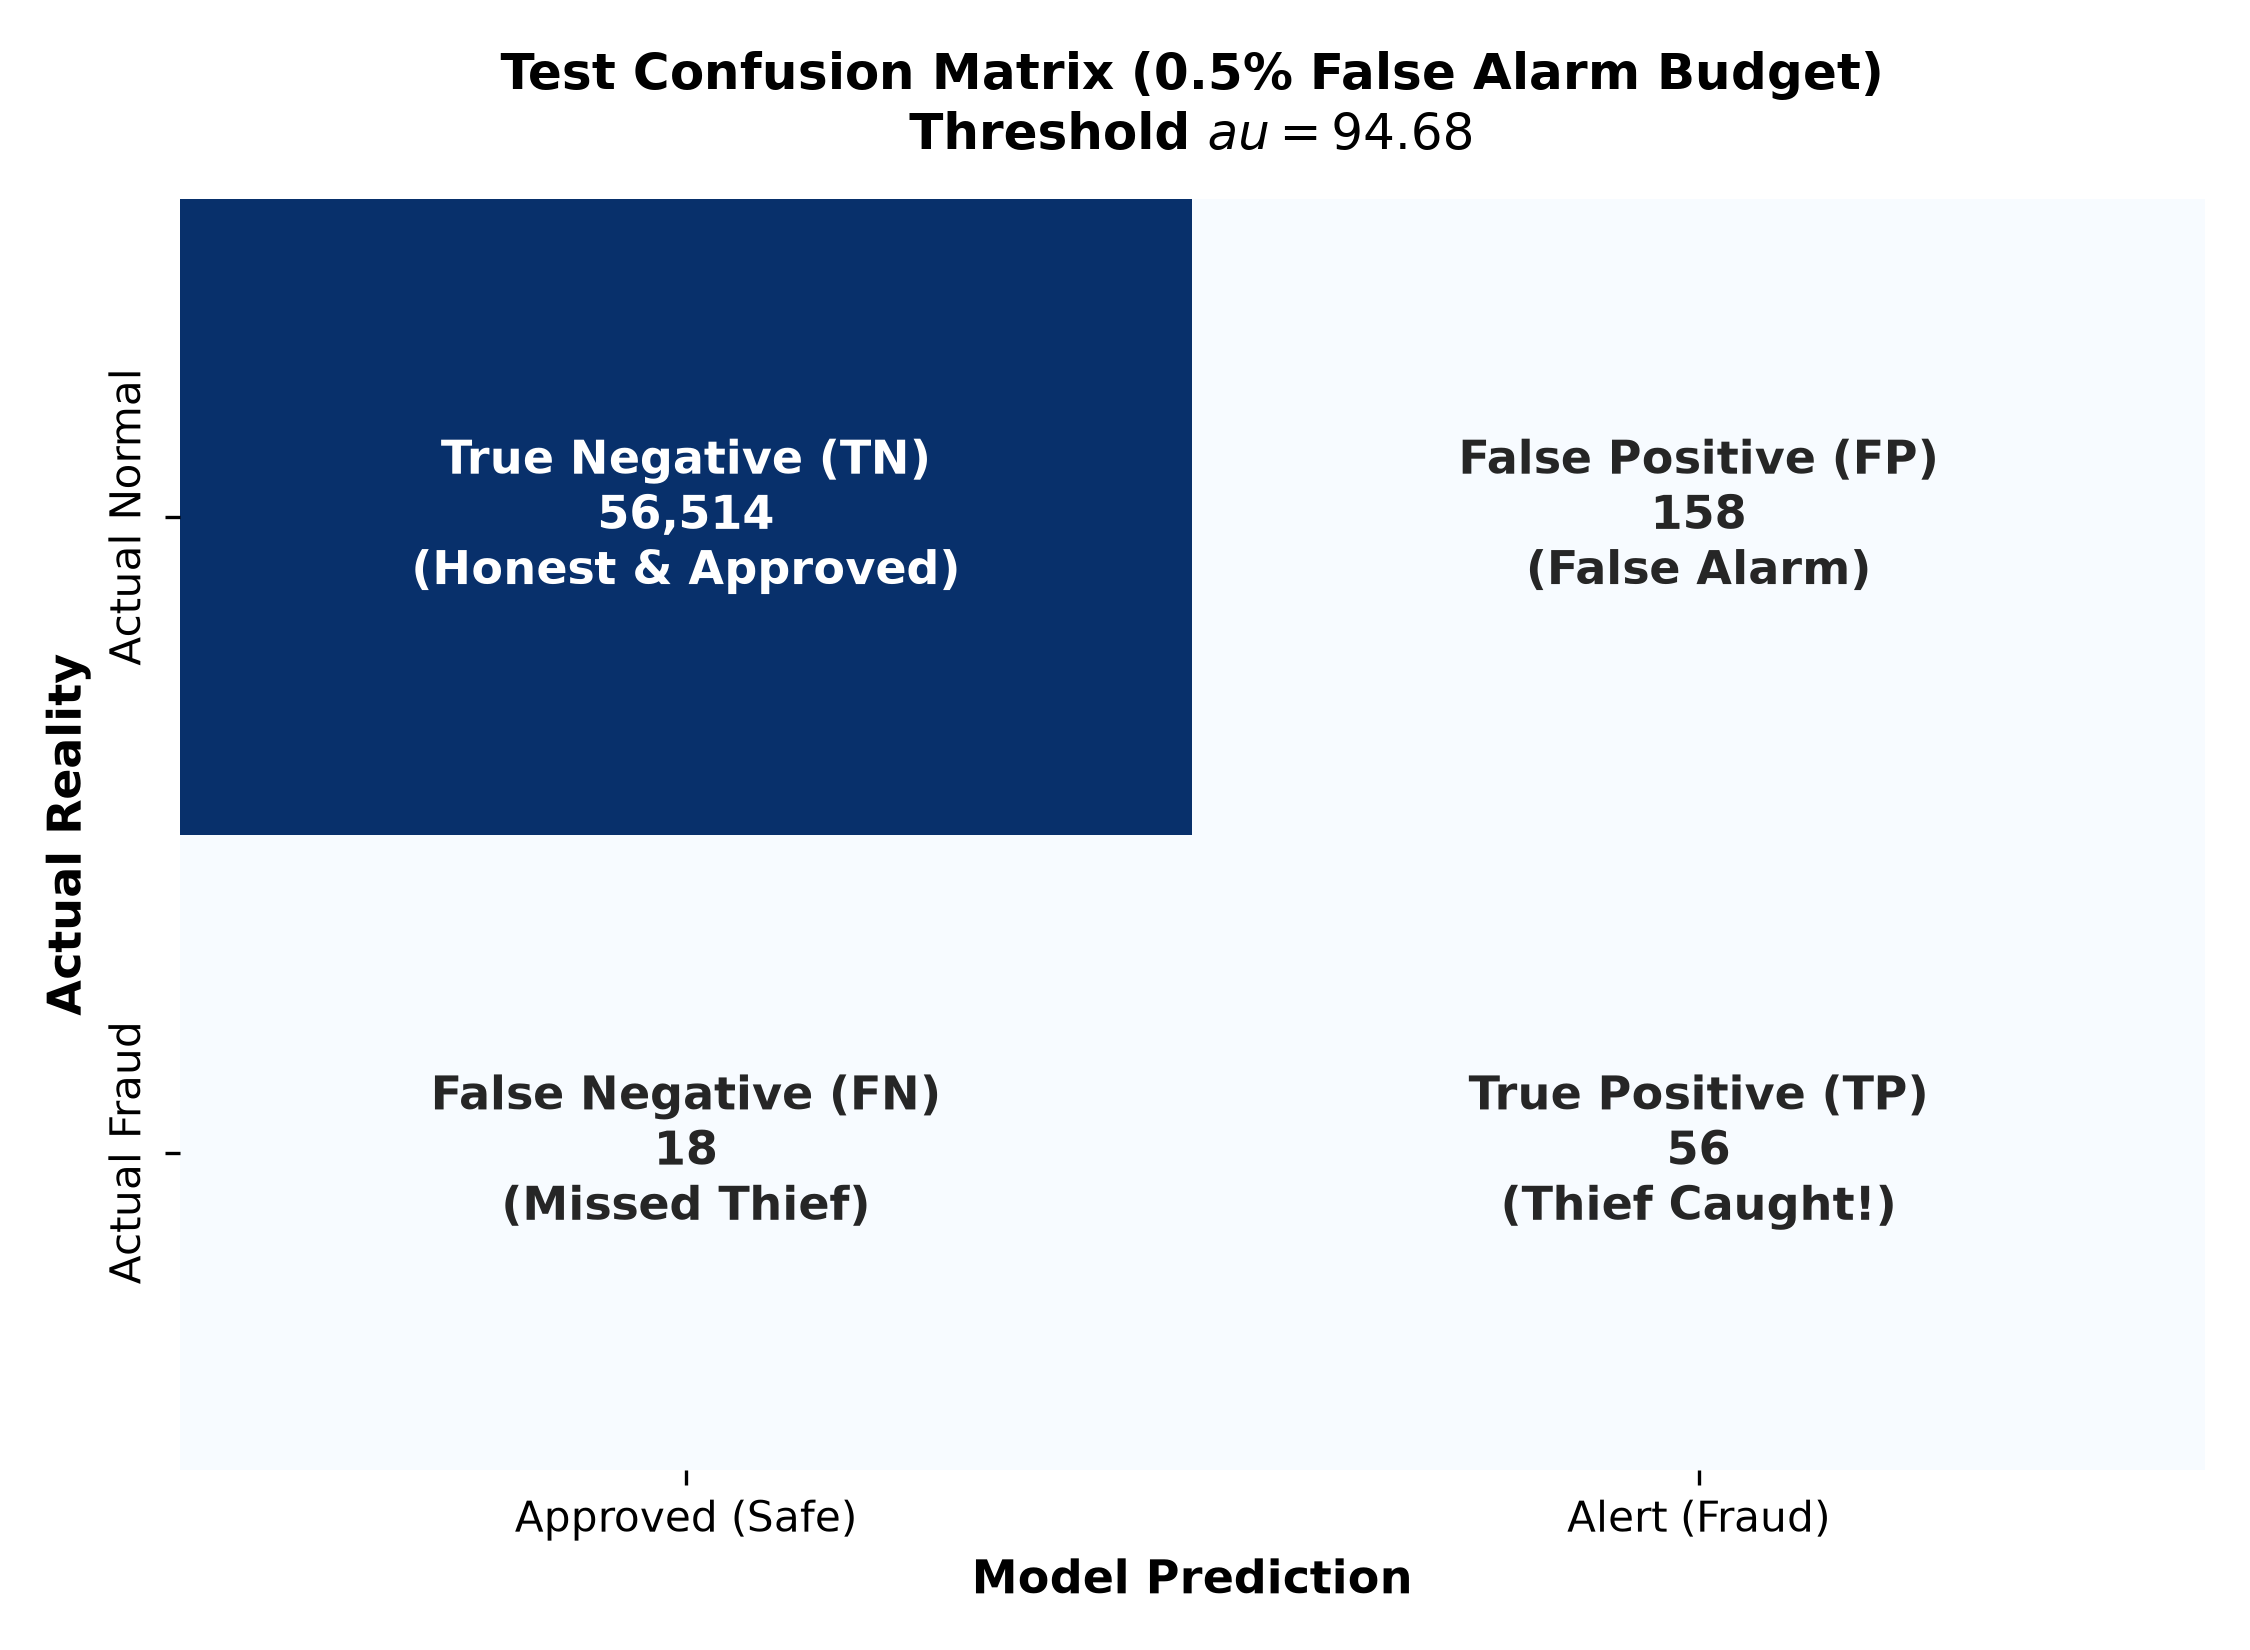
\includegraphics[width=0.85\linewidth]{../results/figures/fig7_gmm_test_confusion_matrix.png}
\caption{Test Confusion Matrix evaluated at the frozen validation threshold $\tau = 94.68$ (0.5\% False Alarm Budget).}
\label{fig:confusion_matrix}
\end{figure}

\subsection{Test Set Evaluation and Operational Impact}
Applying the frozen champion GMM and threshold $\tau = 94.68$ to the 56,746 untouched test transactions yielded the metrics in Table~\ref{tab:test_metrics}.

\begin{table}[t]
\centering
\caption{Out-of-Time Test Performance and 95\% Bootstrap Confidence Intervals}
\label{tab:test_metrics}
\begin{tabular}{lcc}
\toprule
\textbf{Evaluation Metric} & \textbf{Test Value} & \textbf{95\% Bootstrap CI} \\
\midrule
Random Baseline AP & 0.0013 ($0.13\%$) & --- \\
Average Precision (AP) & \textbf{0.6121} & [0.485, 0.743] \\
Trapezoidal PR-AUC & 0.6083 & --- \\
ROC-AUC & \textbf{0.9229} & [0.879, 0.962] \\
Recall @ $\tau = 94.68$ & \textbf{75.68\%} (56/74) & [65.79\%, 84.72\%] \\
Realized False Positive Rate & \textbf{0.28\%} (158/56,672) & --- \\
Precision @ Top 25 Alerts & \textbf{72.00\%} (18/25) & --- \\
Precision @ Top 50 Alerts & \textbf{84.00\%} (42/50) & [70.00\%, 94.00\%] \\
Precision @ Top 100 Alerts & \textbf{56.00\%} (56/100) & --- \\
\bottomrule
\end{tabular}
\end{table}

\subsubsection{Generalization and Stability}
The test Average Precision of **0.6121** aligns closely with the validation score of **0.6661** and falls within the 95\% bootstrap confidence interval $[0.485, 0.743]$. This minimal divergence confirms that the unsupervised density representation learned true behavioral boundaries without overfitting.

\subsubsection{Operational Threshold Verification}
At $\tau = 94.68$, the model intercepts 56 of 74 test frauds (**75.7\% Recall**) while incurring only 158 false alarms out of 56,672 legitimate transactions (**0.28\% False Positive Rate**), safely outperforming the bank's 0.5\% budget (Fig.~\ref{fig:confusion_matrix}).

\subsubsection{Human Review Capacity Triage (Scenario B)}
When evaluating prioritized triage queues, the top 50 highest anomaly scores contain 42 confirmed frauds (**84.0\% Precision**). Investigators reviewing this queue operate with exceptional efficiency, as over 8 out of every 10 investigated alerts are confirmed fraud. Precision naturally moderates to 56.0\% at Top 100 as the pool of available fraud cases (74 total) is progressively exhausted.

\section{Conclusion and Phase 2 Roadmap}
This Phase~1 investigation establishes that unsupervised Gaussian Mixture Models, optimized with multi-seed restarts and full covariance structures, serve as an effective frontline triage mechanism for credit card fraud. By scoring transactions via negative log-likelihood under a model trained purely on legitimate activity, our pipeline achieved an Average Precision of 0.6121 (470$\times$ random guessing), captured 75.7\% of out-of-time fraud within a 0.28\% false-positive budget, and delivered 84.0\% precision in top-50 human review queues.

\textbf{Phase 2 Transition:} In Phase~2 (Deep Learning), we will implement deep autoencoder architectures to benchmark reconstruction error against GMM density scoring. We will conduct systematic ablations across bottleneck dimensions, activation non-linearities, and regularisation schemes, and investigate hybrid ensembles combining autoencoder latent representations with Gaussian mixture density estimation.

\begin{thebibliography}{10}
\bibitem{dalpozzolo2018credit}
A.~Dal Pozzolo, G.~Boracchi, O.~Caelen, C.~Alippi, and G.~Bontempi, ``Credit card fraud detection: A realistic modeling and evaluation framework,'' \emph{IEEE Transactions on Neural Networks and Learning Systems}, vol.~29, no.~8, pp. 3784--3796, 2018.

\bibitem{dalpozzolo2015calibrating}
A.~Dal Pozzolo, O.~Caelen, R.~A. Johnson, and G.~Bontempi, ``Calibrating probability with undersampling for unbalanced classification,'' in \emph{IEEE Symposium Series on Computational Intelligence (SSCI)}, 2015, pp. 159--166.

\bibitem{carcillo2018scarff}
F.~Carcillo, A.~Dal Pozzolo, Y.-A. Le~Borgne, O.~Caelen, Y.~Mazzer, and G.~Bontempi, ``SCARFF: A framework for addressing drift in fraud detection with streaming active learning,'' \emph{Information Sciences}, vol. 465, pp. 252--270, 2018.

\bibitem{chandola2009anomaly}
V.~Chandola, A.~Banerjee, and V.~Kumar, ``Anomaly detection: A survey,'' \emph{ACM Computing Surveys (CSUR)}, vol.~41, no.~3, pp. 1--58, 2009.

\bibitem{bishop2006pattern}
C.~M. Bishop, \emph{Pattern Recognition and Machine Learning}.\hskip 1em plus 0.5em minus 0.4em\relax New York: Springer, 2006.

\bibitem{davis2006relationship}
J.~Davis and M.~Goadrich, ``The relationship between Precision-Recall and ROC curves,'' in \emph{Proceedings of the 23rd International Conference on Machine Learning (ICML)}, 2006, pp. 233--240.

\bibitem{zong2018deep}
B.~Zong, Q.~Song, M.~R. Min, W.~Cheng, C.~Lumezanu, D.~Cho, and H.~Chen, ``Deep autoencoding Gaussian mixture model for unsupervised anomaly detection,'' in \emph{International Conference on Learning Representations (ICLR)}, 2018.

\bibitem{dagostino1973tests}
R.~D'Agostino and E.~S. Pearson, ``Tests for departure from normality. Empirical results for the distributions of $b_2$ and $\sqrt{b_1}$,'' \emph{Biometrika}, vol.~60, no.~3, pp. 613--622, 1973.

\bibitem{massey1951kolmogorov}
F.~J. Massey, ``The Kolmogorov-Smirnov test for goodness of fit,'' \emph{Journal of the American Statistical Association}, vol.~46, no. 253, pp. 68--78, 1951.

\bibitem{sakurada2014anomaly}
M.~Sakurada and T.~Yairi, ``Anomaly detection using autoencoders with nonlinear dimensionality reduction,'' in \emph{Proceedings of the MLSDA 2nd Workshop on Machine Learning for Sensory Data Analysis}, 2014, pp. 4--11.
\end{thebibliography}

\end{document}
